\documentclass{article}
\usepackage[utf8]{inputenc}
\newcommand{\ii}{{\bf i}}
\newcommand{\jj}{{\bf j}}
\newcommand{\kk}{{\bf k}}
\newcommand{\id}{{\bf 1}}
\newcommand{\hur}{\frac{\id+\ii+\jj+\kk}{2}}%The "Hurwitz point"
\newcommand{\hurwitz}{\Z\left[\hur,\ii,\jj,\kk\right]}%The set of Hurwitz integers
\usepackage{wrapfig}
\usepackage[utf8]{inputenc}
\usepackage[dvips]{graphicx}
\usepackage{a4wide}
\usepackage{amsmath}
\usepackage{euscript}
\usepackage{amssymb}
\usepackage{amsthm}
\usepackage{amsopn}
\usepackage[colorinlistoftodos]{todonotes}
\usepackage{graphicx}
\usepackage[T1]{fontenc}
\newcommand\mybar{\kern1pt\rule[-\dp\strutbox]{.8pt}{\baselineskip}\kern1pt}

\usepackage{ulem}
\usepackage{xcolor}
\newcommand{\cs}[1]{\color{blue}{#1}\normalcolor}

%Matrix commands
\newcommand{\ba}{\begin{array}}
\newcommand{\ea}{\end{array}}
\newcommand{\bmat}{\left[\begin{array}}
\newcommand{\emat}{\end{array}\right]}
\newcommand{\bdet}{\left|\begin{array}}
\newcommand{\edet}{\end{array}\right|}

%Environment commands
\newcommand{\be}{\begin{enumerate}}
\newcommand{\ee}{\end{enumerate}}
\newcommand{\bi}{\begin{itemize}}
\newcommand{\ei}{\end{itemize}}
\newcommand{\bt}{\begin{thm}}
\newcommand{\et}{\end{thm}}
\newcommand{\bp}{\begin{proof}}
\newcommand{\ep}{\end{proof}}
\newcommand{\bprop}{\begin{prop}}
\newcommand{\eprop}{\end{prop}}
\newcommand{\bl}{\begin{lemma}}
\newcommand{\el}{\end{lemma}}
\newcommand{\bc}{\begin{cor}}
\newcommand{\ec}{\end{cor}}
\newcommand{\lcm}{\mbox{lcm}}
\newcommand{\defn}{\fbox{definition}}
\newcommand{\prop}{\fbox{proposition}}
\newcommand{\stab}{\mbox{stab}}
\newcommand{\Aut}{\mbox{Aut}}

%sets of numbers
\newcommand{\N}{\mathbb{N}}
\newcommand{\Z}{\mathbb{Z}}
\newcommand{\Q}{\mathbb{Q}}
\newcommand{\R}{\mathbb{R}}

\title{Abstract Algebra}
\author{August, Evelyn}
\date{10/13/2021}

\begin{document}
\maketitle
\fbox{7: proposition} $S_4 \not \cong D_{12}$.\\
\fbox{proof} One of the properties which is preserved through isomorphism is element order. Hence it suffices to show that the number of elements of order $2$ in $S_4$ is not the same as the number of elements of order $2$ in $D_{12}$.\\
By the theorem which states that every permutation can be written in a unique disjoint cycle form, we have the possibilities for elements in $S_4$, and by Ruffini's theorem the orders of these:
$$\begin{array}{cccccc}
     & (\underline{4}) & Order:& 4 & Number: & 6 \\
     & (\underline{3})(\underline{1}) && 3 && 8 \\
     & (\underline{2})(\underline{2}) && 2 && 3 \\
     & (\underline{2})&& 2 && 6 \\
     & (\underline{1})&& 1 && 1 \\
\end{array}$$
Hence there are nine elements in $S_4$ of order $2$.\\

Furthermore, to determine the number of elements in $D_{12}$ of order $2$ it is helpful to think of this geometrically. Since $D_{12}$ is the symmetry group of a 12-sided polygon, it follows that there are $12$ axis of reflection. Reflecting twice about the same axis returns the polygon to its original position, hence each of these vertices is an element in $D_{12}$ with order $2$. Furthermore, rotating by $360/12 = 30$ degrees six times yields the element $R_{180}\in D_{12}$. Rotating by $180$ degrees twice returns the polygon to its original configuration, so the order of $R_{180}$ is $2$. So then there are $12 + 1 = 13$ elements of order $2$ in $D_{12}$. Clearly the number of elements of order $2$ in $D_{12}$ and $S_4$ is not the same, hence they cannot be isomorphic.\\

\fbox{remark} That was a fun problem!\\

\fbox{10: proposition} Let $G$ be a group. Then the mapping $\alpha:G\rightarrow G$ defined $\alpha(g) = g^{-1}$ is an automorphism on $G$ if and only if $G$ is Abelian.\\
\fbox{proof} The proposition is biconditional, so this proof will be broken into two parts. Let $G$ be an arbitrary group and let $\alpha$ be as defined in the proposition. In this proof the group operation will be implied.
\begin{itemize}
    \item[$\Rightarrow$] Suppose that $\alpha$ is an automorphism on $G$. Let $a,b\in G$ be arbitrary elements. By the inverse property of groups, the inverses $a^{-1},b^{-1} \in G$. Then by the closure property of groups, $a^{-1}b^{-1}\in G$, and by definition of $\alpha$, $\alpha(a^{-1}b^{-1}) = (a^{-1}b^{-1})^{-1}$. By the socks shoes property, $(a^{-1}b^{-1})^{-1} = ba$, hence $\alpha(a^{-1}b^{-1}) = ba$. Furthermore, by the supposition that $\alpha$ is an automorphism it follows that $\alpha(a^{-1}b^{-1}) = \alpha(a^{-1})\alpha(b^{-1})= ab$. Substituting, we have $ab = ba$. Since $a,b$ are both arbitrary, it follows that for all $a,b\in G$, $ab = ba$. Then by definition of an Abelian group, $G$ is Abelian.
    \item[$\Leftarrow$] Now suppose that $G$ is Abelian. Let $a$ and $b$ be arbitrary elements in $G$. By the closure property, $ab\in G$. By definition of $\alpha$, $\alpha(ab) = (ab)^{-1}$. By the socks shoes property, $(ab)^{-1} = b^{-1}a^{-1}$. By assumption that $G$ is Abelian, $b^{-1}a^{-1} = a^{-1}b^{-1}$. Furthermore, by definition of $\alpha$, $a^{-1}b^{-1} = \alpha(a)\alpha(b)$. Substituting, $\alpha(ab) = \alpha(a)\alpha(b)$. Since $a$ and $b$ are arbitrary elements in $G$, it follows that this applies for all elements in $G$. Furthermore, since the inverse of an element is unique, the codomain of $\alpha$ is $G$. In other words, $\alpha$ is surjective. It remains to be shown that $\alpha$ is injective. Let $\alpha(a) = \alpha(b)$ for arbitrary $\alpha(a),\alpha(b)\in G$. By definition of $\alpha$, it follows that $a^{-1} = b^{-1}$. Since the inverse is unique, it follows that $a = b$. Hence $\alpha$ is injective and surjective, and hence bijective. Since $\alpha$ is a bijective function from $G$ to $G$ with the property that $\alpha(ab) = \alpha(a)\alpha(b)$ for all $a,b\in G$, it follows that $\alpha$ is an automorphism on $G$.
\end{itemize}

\fbox{27: proposition} Let $r\in U(n)$. Then the mapping $\alpha:Z_n\rightarrow Z_n$ defined $\alpha(s) = sr \mod n$ for all $s\in Z_n$ is an automorphism on $Z_n$.\\

\fbox{proof} Let $n$ be an arbitrary natural number, and let $r\in U(n)$ be an arbitrary element of $U(n)$. Define $\alpha$ as in the proposition, and let $a,b$ be arbitrary elements in $Z_n$. \\

To show that $\alpha$ is an automorphism, we must first verify that $\alpha$ is a bijection. To prove this, we must prove that it is both injective and surjective. \\

To prove that $\alpha$ is injective, let elements $\alpha(a) = \alpha(b)$ for arbitrary $a,b\in Z_n$. By definition of $\alpha$, $ra\mod n = rb\mod n$. Equivalently, $ra \equiv rb \pmod{n}$. By definition of modular congruence,  $n|ra-rb$. Factoring out $r$ we have $n|r(a-b).$ Since $r\in U(n)$, by definition of $U(n)$ $\gcd(r,n) = 1$. By previously proven theorems from number theory and possibly foundations and chapter 0 of the textbook, it follows that $n|a-b$. Then by definition of modular congruence, $a\equiv b \pmod{n}$. In other words, the equivalence classes of $a$ and $b$ are equal, so we have $a = b$. Since $a,b$ are arbitrary, it follows that for all $a,b\in Z_n$ $\alpha(a) = \alpha(b)$ implies $a = b$. By definition of injectivity $\alpha$ is injective.\\

To prove that $\alpha$ is surjective, let $x\in Z_n$ be arbitrary. By the inverse properties of groups, since $r\in U(n)$ and the group operation of $U(n)$ is multiplication of equivalence classes, there exists some element $r^{-1}\in U(n)$ such that $rr^{-1} = 1$. Furthermore, $U(n) \subseteq Z_n$ ($Z_n$ is just the equivalence classes modulo $n$, and $U(n)$ is set of such elements that are relatively prime to $n$). Hence $r^{-1}\in Z_n$. Furthermore, since equivalence classes modulo $n$ are closed under multiplication (as shown in foundations and number theory), $r^{-1}x\in Z_n$. Then $x = rr^{-1}x = \alpha(r^{-1}x)$. So there exists some element in $Z_n$ which $\alpha$ maps to $x$. Since $x$, is arbitrary, this applies to all elements in $Z_n$. Then by definition of surjectivity $\alpha$ is surjective. Since $\alpha$ is injective and surjective, it follows that $\alpha$ is bijective. \\


Then we take two elements, $a,b\in Z_n$ , and show that $\alpha(a+b) = \alpha(a) + \alpha(b).$ By the distributive law in $\Z_n$, we get the following:  $\alpha(a+b) = r(a+b) \mod n = (ra + rb) \mod n$. Hence, by definition of $\alpha$, $\alpha(a+b)=\alpha(a)+\alpha(b)$. \\

Now to show that the bijection $\alpha: Z_n\rightarrow Z_n$ is an automorphism on $Z_n$. Let $a$ and $b$ be arbitrary elements in $Z_n$. 

\fbox{45: proposition} Suppose that $g$ and $h$ induce the same inner automorphism on a group $G$. Then $h^{-1}g\in Z(G)$.\\

\fbox{proof} By supposition $\phi_g = \phi_h$. By definition of function equality it follows that for all $a\in G$, $\phi_g(a) = \phi_h(a)$. Let $a$ be an arbitrary element in $G$. By definition of the inner automorphism, $\phi_g(a) = gag^{-1}$ and $\phi_h(a) = hah^{-1}.$ By supposition that $\phi_g$ and $\phi_h$ are equal, $gag^{-1} = hah^{-1}.$ Operating $h^{-1}$ both sides on the left, we have $h^{-1}gag^{-1} = h^{-1}hah^{-1} = ah^{-1}.$ Operating $g$ both sides on the right we have  $h^{-1}gag^{-1}g = ah^{-1}g$. Then $h^{-1}ga = ah^{-1}g$. Since $a$ is arbitrary, it follows that for all $a\in G$, $h^{-1}g a = a h^{-1}g$. By definition of the center of a group, $h^{-1}g \in Z(G)$. \\
\newpage

\fbox{15, proposition} Let $G$ be a group. The sets $\Aut(G)$ and Inn(G) form a group under function composition.\\

\fbox{proof} To show that $\Aut(G)$ is a group, we must show that it satisfies the group axioms. First, we must show that this is nonempty. Consider the identity map on $G$, $1_G:G\rightarrow G$. By theorems from foundations $1_G$ is bijective. Furthermore, $1_G(ab) = ab = 1_G(a) 1_G(b),$ as follows from the definition of the identity map. Then by definition of an automorphism, $1_G$ is an automorphism on $G$. Hence $1_G\in \Aut(G)$. \\

Now to show that $\Aut(G)$ satisfies the identity property. Let $\alpha \in \Aut(G)$ for some arbitrary $\alpha:G\rightarrow G$. Then $\alpha\circ 1_G(a) = \alpha(1_G(a)) = \alpha(a) = 1_G(\alpha(a)) = 1_G\circ \alpha(a).$ Then by definition of function equality $1_G\circ \alpha = 1_G = \alpha\circ 1_G$. Hence $1_G$ is the identity in $\Aut(G)$ and $\Aut(G)$ satisfies the identity property of groups. As for Inn(G), consider the function $\Phi_e(x)=exe^{-1}=x$ for all $x\in G$. \\

To show that $\Aut(G)$ satisfies the inverse property, let $\alpha\in \Aut(G)$ be an arbitrary automorphism on $G$. By definition of automorphisms, there exists some inverse function $\alpha^{-1}:G\rightarrow G$ such that $\alpha^{-1}\circ \alpha = 1_G = \alpha\circ 1_G$. As we know from foundations that $\alpha^{-1}$ is bijective, it remains to be shown that $\alpha^{-1}$ is operation preserving. To verify this, let $a,b\in G$ be arbitrary. By construction of $\alpha$ as an automorphism, and since by definition of inverse functions, $\alpha\circ \alpha^{-1}(a+b) = 1_G(a+b) = a+b = \alpha(\alpha^{-1}(a)) + \alpha(\alpha^{-1}(b)).$ Since $\alpha$ is an isomorphism and hence is operation preserving, we have $\alpha\circ\alpha^{-1}(a+ b) = \alpha(\alpha^{-1}(a) + \alpha^{-1}(b)).$ Composing $\alpha^{-1}$ on the left on both sides, we have $\alpha^{-1}(a+b) = \alpha^{-1}\circ \alpha(\alpha^{-1}(a) + \alpha^{-1}(b)) = \alpha^{-1}(a) + \alpha^{-1}(b)$. Hence $\alpha^{-1}$ is a bijective function from $G$ to $G$ that is operation preserving, so it is an automorphsim, and hence $\alpha^{-1}\in \Aut(G)$. Since $\alpha$ is an arbitrary element in $\Aut(G)$, it follows that all elements in $\Aut(G)$ have an inverse.\\

To show that $\Aut(G)$ is closed under function composition, consider two elements $\alpha$ and $\beta$ in $\Aut(G)$. Since by construction $\alpha$ and $\beta$ both map from $G$ to $G$, the composition is well defined. Furthermore, recall from foundations that the composition of two bijective functions is bijective, hence $\alpha\circ\beta$ is bijective. It remains to be shown that $\alpha\circ\beta$ is operation preserving. Let $a, b\in G$ be arbitrary. Since $\beta$ is operation preserving, it follows that $\beta(a+b) = \beta(a)+\beta(b)$. Furthermore, $\beta(a),\beta(b)\in G$ by definition of $\beta$. Then $\alpha\circ\beta(a+b) = \alpha(\beta(a+b)) = \alpha(\beta(a) + \beta(b)) = \alpha(\beta(a)) + \alpha(\beta(b)) = \alpha\circ\beta(a) +\alpha\circ\beta(b).$ Since $a,b\in G$ and are arbitrary, it follows that for all $a,b\in G$ $\alpha\circ \beta(a+b) = \alpha\circ\beta(a) + \alpha\circ\beta(b)$. Hence $\alpha\circ\beta$ is a bijective, operation preserving map from $G$ to $G$, hence $\alpha\circ\beta\in \Aut(G)$. Since $\alpha$ and $\beta$ are arbitrary elements in $\Aut(G)$, it follows that for all $\alpha$ and $\beta$ in $\Aut(G)$, $\alpha\circ \beta\in \Aut(G)$. Hence $\Aut(G)$ is closed under function composition.\\

Finally, since the group operation is function composition, which is associative, it follows that $\Aut(G)$ under function composition satisfies the associative property.\\

Since $\Aut(G)$ under function composition is a nonempty set that satisfies the identity, inverse, closure, and associative properties, it follows that $\Aut(G)$ is a group.\\

Furthermore, to show that Inn(G) is a group, let us first show that it satisfies the identity property, which implies then that Inn(G) is nonempty. Consider the function $\Phi_e(x)=exe^{-1}=x$ for all $x\in G$, with e denoting the identity element in G. In order to show that $\Phi_e(x)$ is bijective, we must show that it is injective and surjective. First, suppose $\Phi_e(a)=\Phi_e(b)$ for some arbitrary a and b in G. By definition of $\Phi_e$, it follows that $eae^{-1}=ebe^{-1}$ and by definition of the identity element e, it follows that $a=b$. Thus $\Phi_e$ is injective. Second, let a be an arbitrary element in G. By definition of the identity element in G and of $\Phi_e$, it follows that $a=eae^{-1}=\Phi_e(a)$, thus a is mapped to itself. Since a is arbitrary, it follows that $\Phi_e$ is surjective, and hence $\Phi_e$ is bijective. Furthermore, for some arbitrary a and b in G, consider $\Phi_e(ab)=eabe^{-1}=eae^{-1}ebe^{-1}=\Phi_e(a)\Phi_e(b)$. Hence, it follows that $\Phi_e$ is an automorphism. In order to show that $\Phi_e$ is the identity element, consider the function composition $\Phi_e \circ \Phi_a(x)$ for some arbitrary $\Phi_a \in$ Inn(G). By properties of G it follows that $\Phi_e(\Phi_a(x))=\Phi_e(axa^{-1})=eaxa^{-1}e^{-1}=axa^{-1}=aexe^{-1}a^{-1}=\Phi_a(\Phi_e(x))=\Phi_a \circ \Phi_e(x)=\Phi_a(x)$. Thus, function composition is preserved and $\Phi_e$ is the identity element in Inn(G), which implies that Inn(G) is nonempty. \\

In order to show that Inn(G) satisfies the inverse property, let $\Phi_a$ be an arbitrary element in Inn(G). By definition of automorphisms, $\Phi_a$ is bijective, hence by theorems from foundations there exists some inverse function $\Phi_a^{-1}: G \rightarrow G$, such that $\Phi_a \circ \Phi_a^{-1} =\Phi_a^{-1} \circ \Phi_a = \Phi_e$. By the socks-shoe-property, it follows that $\Phi_a \circ \Phi_a^{-1} =axa^{-1}(axa^{-1})^{-1}=axa^{-1}ax^{-1}a^{-1}=e=(axa^{-1})^{-1}axa^{-1}=\Phi_a^{-1} \circ \Phi_a = \Phi_e$. The inverse function of a bijective function is bijective as well, thus it only remains to show that it is operation preserving. However, we know that by Thm 6.3 the inverse function of an isomorphism is an isomorphism. Hence, Inn(G) satisfies the inverse property.\\

In order to show closure, let $\Phi_a \and \Phi_b \in$ Inn(G) be arbitrary. Consider $\Phi_a \circ \Phi_b(x)=\Phi_a(\Phi_b(x))=abxb^{-1}a^{-1}=\Phi_{ab}(x)$, since $ab \in G$ by the closure property of G. Thus, $\Phi_ab \in$ Inn(G) and Inn(G) is closed under function composition. \\

Lastly, function composition is associative by definition. Inn(G) satisfies all the group properties and hence Inn(G) is a group.\\ 
\newpage
\\

\fbox{challenge problem} Given $i^2 = j^2 = k^2 = ijk = -1$, find the cayley table for elements in $\pm\{1,i,j,k\}  = S$.\\
A few observations should make this simpler. First, note that although the set is not commutative, $-1,1$ commute with all elements. Hence, if we know the negative combination of two elements, we also know the positive combination.\\

aMultiplying $k$ on the left on both sides, we have $ijkk =-ij= -k$. So $ij = k$ as well.  \\

Multiplying $j$ on both sides on the right, we have $-ijj = -ijj = -kj = i$. So $-i = kj$ as well.\\

Multiplying $k$ on both sides on the left we have $-ki = kkj = -j$. Hence $j = ki$ as well. To find $ik$, multiply $i$ on both sides, yielding $iji = ikii = -ik$. But since $ij = k$, $ki = -ik$. But we know this too, so $j = -ik$. This is really interesting how things start to connect. As in the last problem, I found the Cayley table started to fill in itself as I started to learn rules about the group.\\

\begin{figure}{0.5\textwidth}
    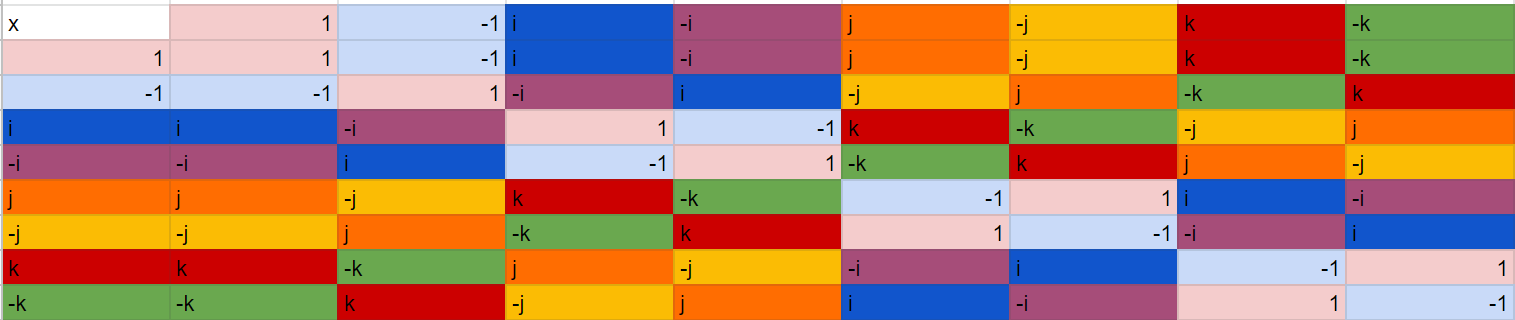
\includegraphics[width=1\textwidth]{cayley_quaternions.png}
  \caption{cayey table}
\end{figure}
\fbox{observation} Any time we have $ab = c$ for some $a,b,c\in S$, we also have $(-a)b = -c$, $(-a)(-b) = c$, $(a)(-b) = -c$. In other words, once we know one combination, we also know four others. Furthermore, it is easy to see that $1$ is the identity. This can also be rigorously proven, as $i^2 = -1 = j^2 = k^2$. If we multiply by $i,j,k$ respectively, we get $i^3= i(ii) = i(-1) = -i.$ So we need only change the sign for the -1 columns and rows. So we have eliminated 2 rows and 2 columns, leaving 6x6 = 36 elements. So there are 36/4 = 9 distinct computations \\
\\
\fbox{observation} The cyclic subgroups and their orders should be $<1>:1,<-1>:2,<i>:4,<j>:4,<k>:4,S:8$. The center should be $<-1>$, as these elements commute with all the other elements, but this is not a distinct subgroup. Furthermore, $<1>$ is a subgroup of $<-1>$ and everything else, but $<-1>$ is a subgroup of everything else too. $<i>$, $<j>$, $<k>$ are subgroups of $S$. Furthermore, these are the only subgroups. Suppose on the contrary we had some subgroup containing elements not in the intersection of two other subgroups. Then $i,j$ would be in there, and by the relation we could get $1,-1,-i,-j,k,-k$ as well, so any other set would not be closed. So the subgroup lattice is this:\\
\begin{figure}[htbp]
\centerline{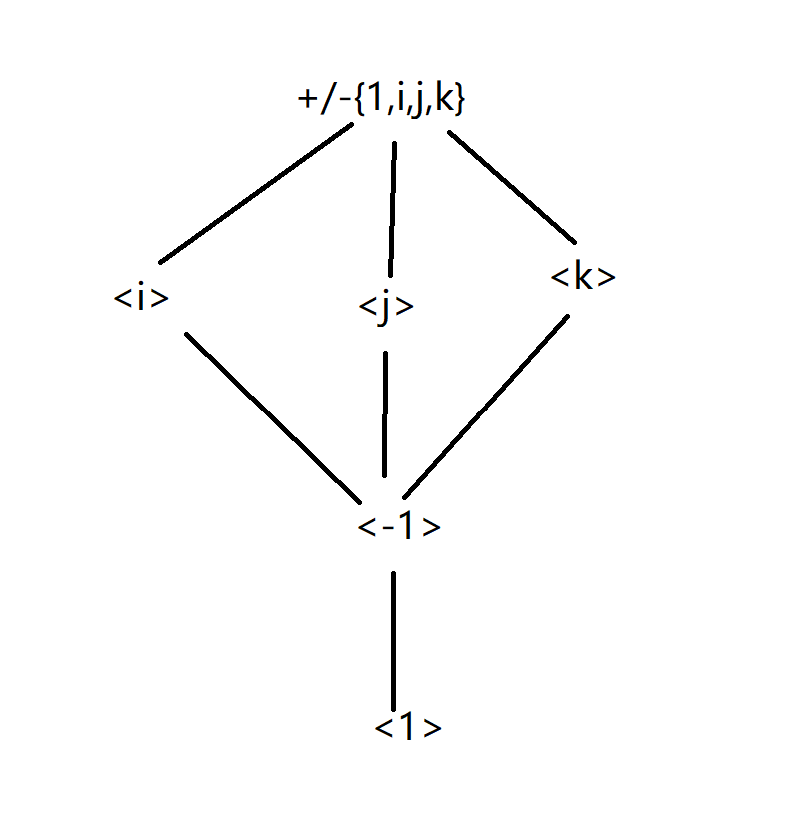
\includegraphics[scale=0.5]{quaternion_latice.png}}
\caption{subgroup lattice}
\label{fig}
\end{figure}
I don't know why this went so far down.\\

Define the set of permutations $G= \{\sigma_a:S\rightarrow S; a\in S\}$ defined $\sigma_a(b) = ab$. This, as shown in the proof of Cayley's theorem, is a group of permutations under function composition which is isomorphic to $S$ under multiplication.\\

The elements of $G$ can be easily determined, as we can simply number the elements on the Cayley table, and show where each element goes, and where that element goes, and so forth. Hence we have $\sigma_1 = (1)$, $\sigma_2 = (12)(34)(56)(78)$, $\sigma_3 = (13)(24)(5768)$, $\sigma_4 = (14)(23)(5867)$, $\sigma_5 = (1526)(37)(48)$, $\sigma_6 = (1625)(38)(47)$, $\sigma_7 = (1728)(3546)$, $\sigma_8 = (1827)(3645).$
\end{document}